% !TEX root = ../main.tex
\chapter{Semantic Web}
\label{ch:semantic_web}

\nocite{rdf_introduction}
In this chapater will follow a brief description of the concept of ontology and of Semantic Web as defined by W3C. This chapter will then furter detail the ontologies and metadata schemata used in the thesis project, namely Semantic Sensor Network (SSN) and Brick.
It is to note that the work presented in this thesis is not directly using all of these technologies, but it draws from their key concepts to reach some goals. It is therefore worth to mention such concepts here.

\section{Introduction to the Semantic Web}
Semantic Web is a term that identify an evolution of the web in which every resource available through the web is associated with a semantic meaning. Semantic Web technologies enable people to create data stores on the Web, build vocabularies, and write rules for handling data.
Semantic web layers are defined by W3C as:
\begin{itemize}
  \item linked data
  \item vocabularies
  \item query
  \item inference
\end{itemize}

\subsection{Linked data}
Linked Data lies at the heart of what Semantic Web is all about: large scale integration of, and reasoning on, data on the Web. To make the Web of Data a reality, it is important to have the huge amount of data on the Web available in a standard format, reachable and manageable by Semantic Web tools. Furthermore, not only does the Semantic Web need access to data, but relationships among data should be made available, too, to create a Web of Data (as opposed to a sheer collection of datasets). This collection of interrelated datasets on the Web can also be referred to as Linked Data.

\subsubsection{Resource Description Framework} \label{subsec:rdf}
RDF \cite{rdf_standard} is a description language, which aims to capture the semantics of data represented on the Web. The RDF standard is based on several fundamental concepts. The first such concept is ``resource''. Resources are the basic objects, or ``things'', that are to be described in the domain (e.g. rooms, floors, sensors etc.). All resources are identified through a unique, global identifier called the universal resource identifier (URI). In most applications, the URI is the uniform resource locator (URL) of a Web page, a part of a Web page, or a link to a document available on a Web server. However, the URI is a more general concept, the only condition is that it uniquely identifies a resource. Examples of resources could be ``unibs:florenzi.002'' as well as ``unibs:thesis1234'', or ``https://www.w3.org/RDF/''.  Another essential concept is ``property''. Properties describe relations between resources and following the previous example we could say that ``has\textunderscore author'', ``has\textunderscore name'', ``has\textunderscore subject'' are properties.  Having defined both resources and properties, statements can be derived. Statements, also known as triples, in RDF have the basic form: subject-predicate-object, where the subject is an RDF resource, the predicate is a RDF property, and the object is another RDF resource or a literal (a name, a number, code, etc.). Still referring to the example, the statements could be ``unibs:thesis1234 has\textunderscore author unibs:florenzi.002'', ``unibs:thesis1234 has\textunderscore subject \url{https://www.w3.org/RDF}'' and ``unibs:florenzi.002 has\textunderscore name ``Fabio Lorenzi''''.
RDF data models end up being represented as graphs where subjects and objects are nodes while properties are the edges. The resulting graph, given the RDF notation, in the example is shown in \autoref{fig:rdf_example}.

\begin{figure}
  \centering
  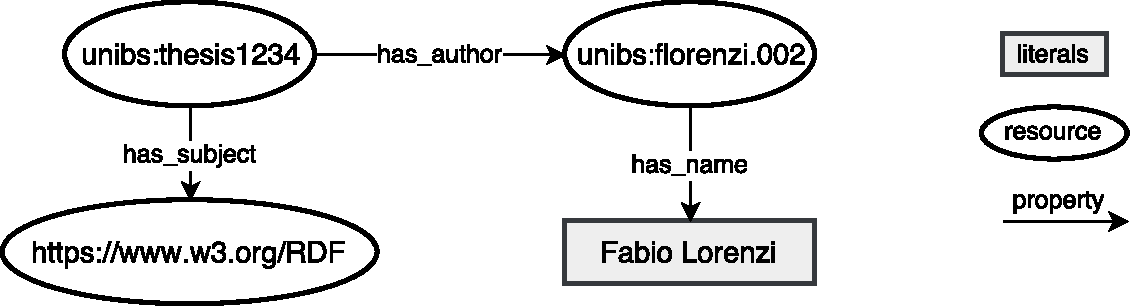
\includegraphics[width=0.8\textwidth]{rdf_example.pdf}
  \caption{Graph representation of the example RDF model}
  \label{fig:rdf_example}
\end{figure}

It is to note that RDF is a conceptual model for representing linked data, but as far as it goes, no semantic is implied in this representation, looking at this model is impossible to understand the meaning of the resources or property, nor to understand if those elements reflect and adhere to rules of a particular domain.
In the example above there is no explicit information telling us that the resource ``unibs:florenzi.002'' is a person and that ``the unibs:thesis1234'' is a book. Furthermore the RDF model represented with ``unibs:florenzi.002 has\textunderscore author unibs:thesis1234'', ``unibs:florenzi.002 has\textunderscore subject \url{https://www.w3.org/RDF}'' and ``unibs:thesis1234   has\textunderscore name ``Fabio Lorenzi'''', yelding the graph representation in \autoref{fig:wrong_rdf_example}, is perfectly fine, altough not semantically correct\footnote{from a common sense point of view. No semantic is explcitly declared}.
Adding semantic to an RDF model, that is detailing the domain ontology, is left to other frameworks as explained in \textbf{\autoref{subsec:vocabularies}}.

\begin{figure}
  \centering
  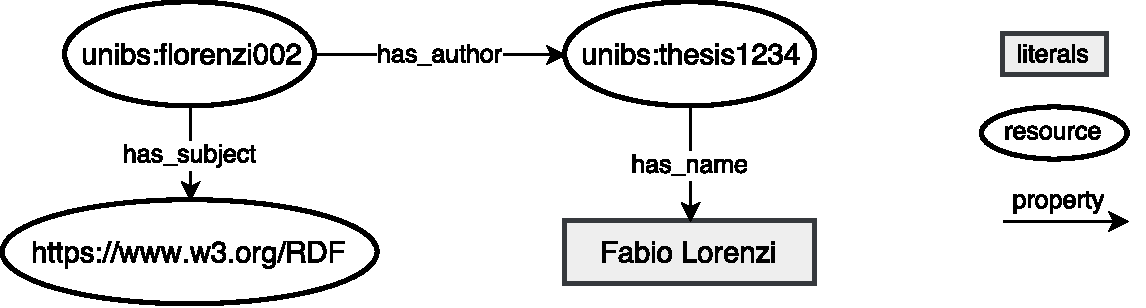
\includegraphics[width=0.8\textwidth]{wrong_rdf_example.pdf}
  \caption{Correct RDF model with wrong semantic}
  \label{fig:wrong_rdf_example}
\end{figure}

\subsection{Vocabularies} \label{subsec:vocabularies}
On the Semantic Web, vocabularies define the concepts and relationships (also referred to as ``terms'') used to describe and represent an area of concern. Vocabularies are used to classify the terms that can be used in a particular application, characterize possible relationships, and define possible constraints on using those terms. There is no clear division between what is referred to as ``vocabularies'' and ``ontologies''. The trend is to use the word ``ontology'' for more complex, and possibly quite formal collection of terms, whereas ``vocabulary'' is used when such strict formalism is not necessarily used or only in a very loose sense. Vocabularies are the basic building blocks for inference techniques on the Semantic Web.

\subsubsection{Resource Description Framework Schema}
RDFS defines a set of RDF resources useful for the description of other RDF resources and properties. Through RDFS it's possible to define and detail the semantic of a RDF model. Among the various concepts introduced with RDFS there are
\begin{itemize}
  \item rdfs:Resource: everything that is described in RDF is a resources
  \item rdfs:Literal: it is text string
  \item rdfs:Property: it represent the properties
  \item rdfs:Class: it is similar to the concept of type or class in an object oriented programming language.
  \item rdfs:subClassOf: it specify inheritance, eventually multiple, between classes.
  \item rdfs:range: it tells which resources are permitted as object in a statement
  \item rdfs:domain: it tells which resources are permitted as subject in a statement
\end{itemize}

it is to note that the RDFS is a RDF model itself and it's used for explicitly declare the domain knowledge of a given RDF model. We refer to the RDFS as an ontology and to the RDF model as the instances of such ontology.
Following RDFS, it is possible to model domain knowledge for the example in \textbf{\autoref{subsec:rdf}} as in \autoref{fig:rdfs_ontology}.

\begin{figure}
  \centering
  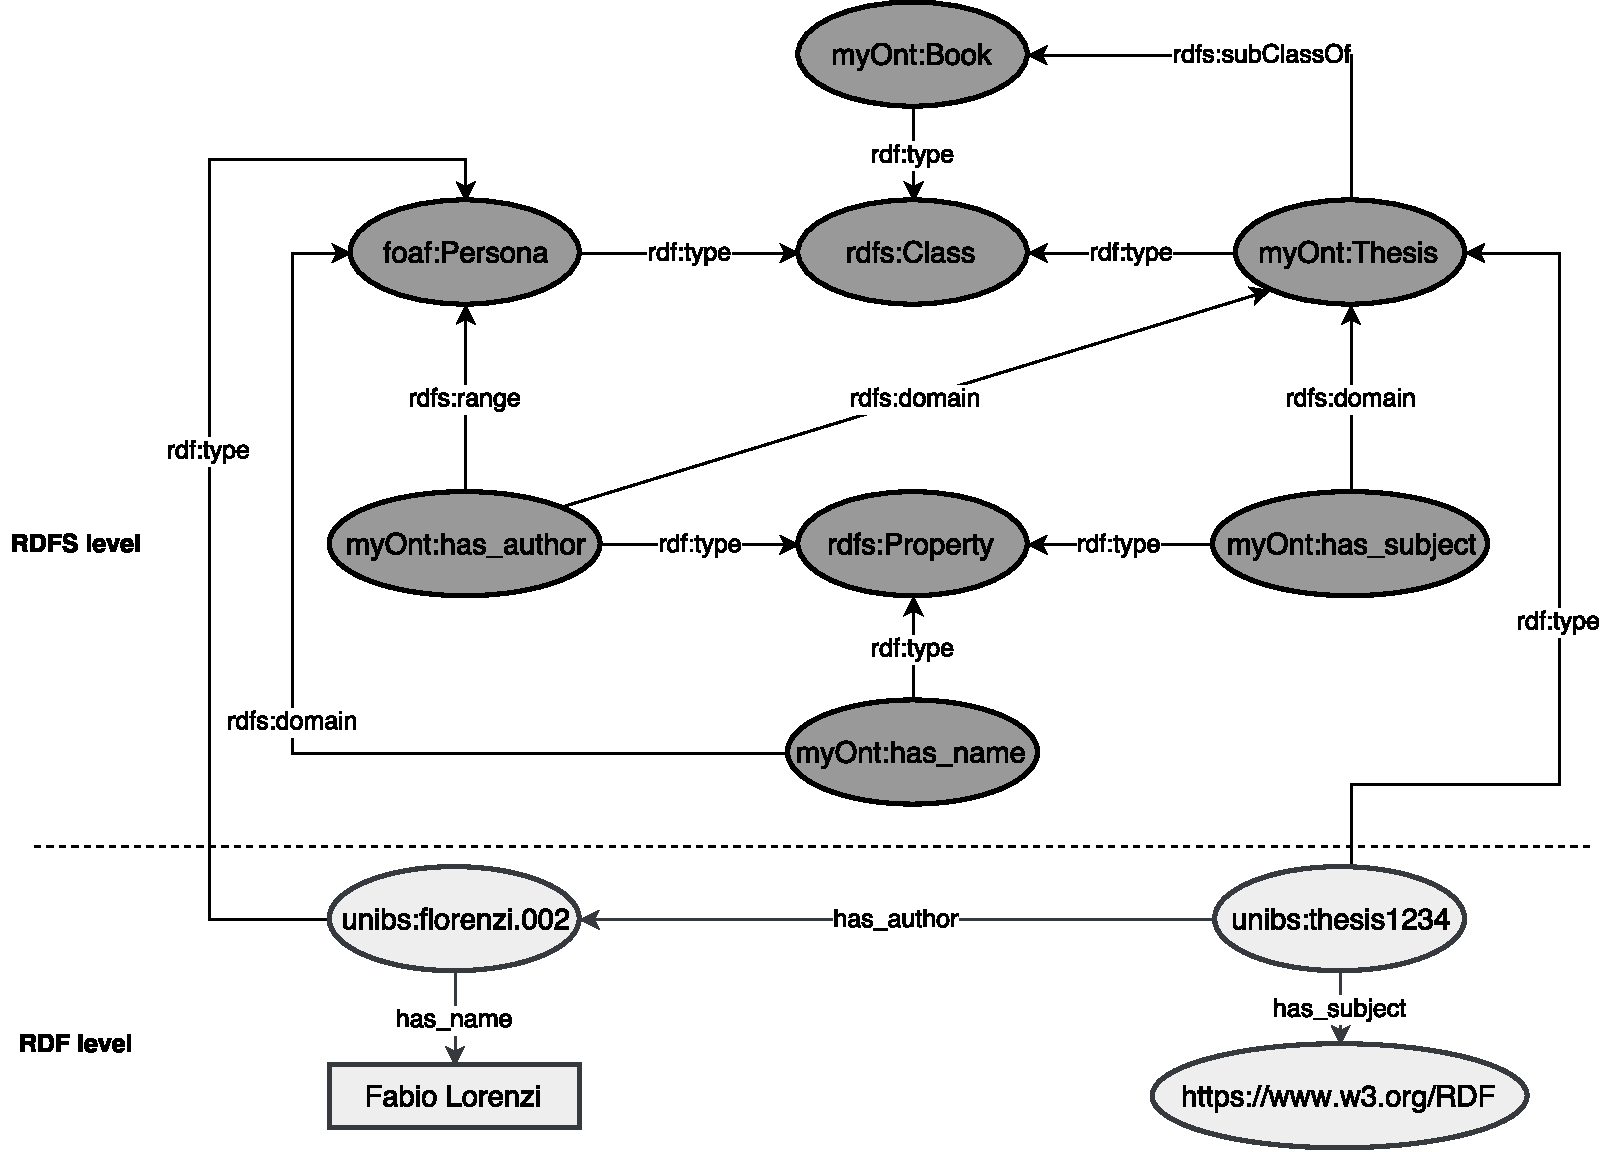
\includegraphics[width=0.9\textwidth]{rdfs_example.pdf}
  \caption{RDFS representation of an ontology}
  \label{fig:rdfs_ontology}
\end{figure}

This ``layering'' approach is what allows for the design of reusable ontologies and gives opportunity to automatically infer new knowledge based on the RDFS model of the data.
Still looking back at the example, lets suppose that the statement ``unibs:florenzi.002 rdf:type foaf:Person'' wasn't in the ground knowledge of the RDF model. Even without this explicit information wasn't available, a reasoner would have been able to infer that statement (dotted line) given the semantic description of the property ``myOnt:has\textunderscore author'' (bold line). The process is represented in \autoref{fig:inference_rdfs}.

\begin{figure}
  \centering
  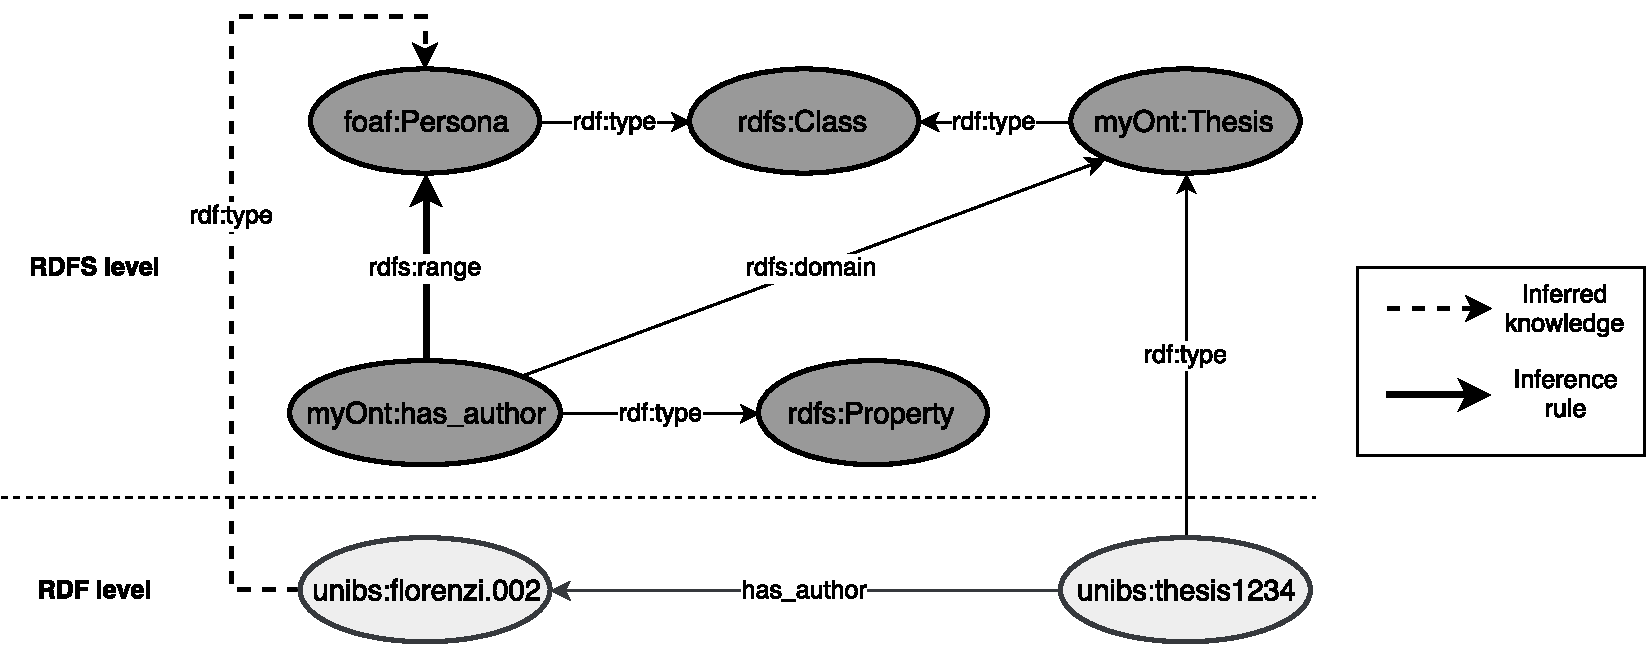
\includegraphics[width=1\textwidth]{inference_rdfs.pdf}
  \caption{Inference process of new knowledge}
  \label{fig:inference_rdfs}
\end{figure}

\subsection{Query}
Just as relational databases or XML need specific query languages (SQL and XQuery), the Web of Data, typically represented using RDF as a data format, needs its own, RDF-specific query language and facilities.

\subsubsection{SPARQL Protocol and RDF Query Language}
A mean for querying RDF models is defined by SPARQL \cite{sparql_reccomendation} query language. Technically, SPARQL queries are based on (triple) patterns. As RDF can be seen as a set of relationships among resources, SPARQL queries provide one or more patterns against such relationships. These triple patterns are similar to RDF triples, except that one or more of the constituent resource references are variables. A SPARQL engine would returns the resources for all triples that match these patterns. To represent a pattern (or query) to run against the data model, SPARQL define a series of keywords % TODO something about SPARQL

\section{Ontologies for smart buildings}
\subsection{Brick} \label{subsec:brick}
Brick schema \cite{brick_schema} defines domain specific concepts aimed at describing sensors in a building with its context. It is composed of three parts
\begin{itemize}
  \item a class hierarchy of entities describing various building subsystems
  \item a minimal set of relationships for connecting entities
  \item a methods for encapsulation in the form of Function Blocks
\end{itemize}

the main concept in Brick is the concept of tag introduced with project Haystack \cite{project_haystack}, which is further enriched by an ontology that cristallizes the concepts defined by tags. A tag is a flexible framework for annotating metadata to building data points. In Brick tags are grouped together as sets, named tagset, to represent entities; the tags {room}, {temperature} and {sensor} can be grouped together as {room temperature sensor} representing a single entity. The concept of tagset is well integrated with the class hierarchy concept of the ontologies: a {room temperature sensor} is a subclass of a generic {temperature sensor}.
As the main goal of Brick is to represent points in a building's BMS, Points is one of the main classes of Brick, which subclasses define specific type of points like Sensor. The most common concepts a Point can be related to are Location, Equipement and Measurement so those classes, together with the Point class, form the core classes of Brick. Those classes are further subclassed to form a hierarchy able to comprehend every entity of a building. Alongside classes, relationships play a crucial role in connecting entities and thus providing a context for many applications. Brick designed a set of minimal, intuitive and multipurpose relationship fundamental in capturing existing relationship. \autoref{fig:brick_schema} shows the Brick core concepts and the designed set of relationships.

\begin{figure}
  \centering
  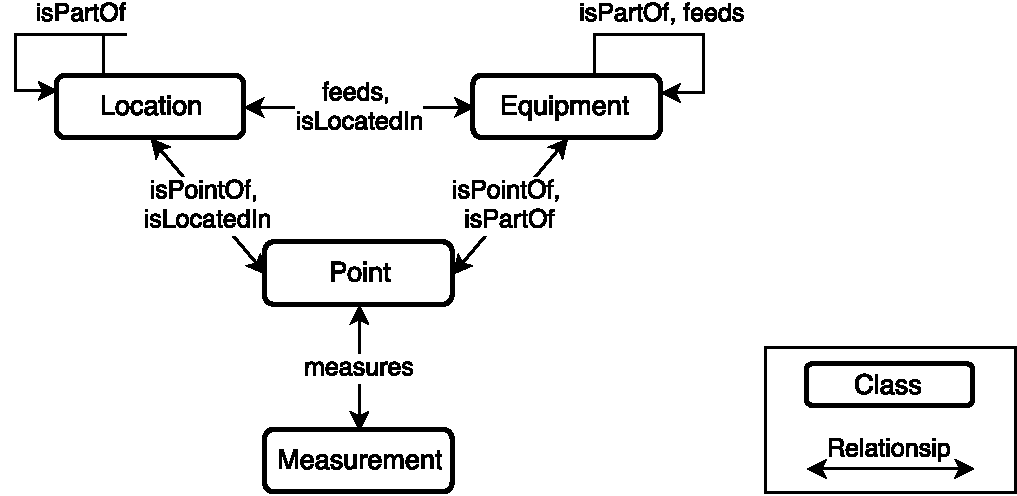
\includegraphics[width=0.7\textwidth]{brick_schema.pdf}
  \caption{Brick schema core concepts}
  \label{fig:brick_schema}
\end{figure}

\subsection{Semantic Sensor Network ontology} \label{subsec:ssn}
While Brick schema was used to model the building domain, the Semantic Sensor Network (SSN) ontology \cite{ssn_ontology} was chosen because it provides a different view of the various aspect of the sensing process, beyond the specific building domain. Peculiar to the SNN Ontology (SSNO) is the Stimulus-Sensor-Observation design pattern.
This pattern differentiate between the concept of ssn:Sensor for physical devices that take measurements in form of ssn:Observation and ssn:Stimulus that is the actual change in the enviroment that caused a particular observation, so that it possible to differentiate that stimuli occur in the reality even if no sensor is monitoring them, thus modeling unobservabel states of a system, and that observation made from a sensor can be different from the real event (e.g errors, failures, noise ). These concepts aside, SSN provide other useful classes that are ssn:FeatureOfInterest that represent generic entities which status is to be monitored, like rooms, fans or floors and ssn:Property that embodies specific physical quantities that a sensor ought to monitor. All the classes are connected by a set of relationships that are ssn:hasProperty that connects a ssn:FeatureOfInterest with meaningful physical properties, like a temperature in a room; ssn:isProxyFor represent that a given ssn:Stimulus influence a ssn:Property as in ``another occupant in a room raises its temperature''; ssn:includeEvent create a dependency between an observation and a event that causes it; ssn:observedBy links an observation to the sensor that could measure it. \autoref{fig:ssn_ontology} show the resulting SSN ontology.

\begin{figure}
  \centering
  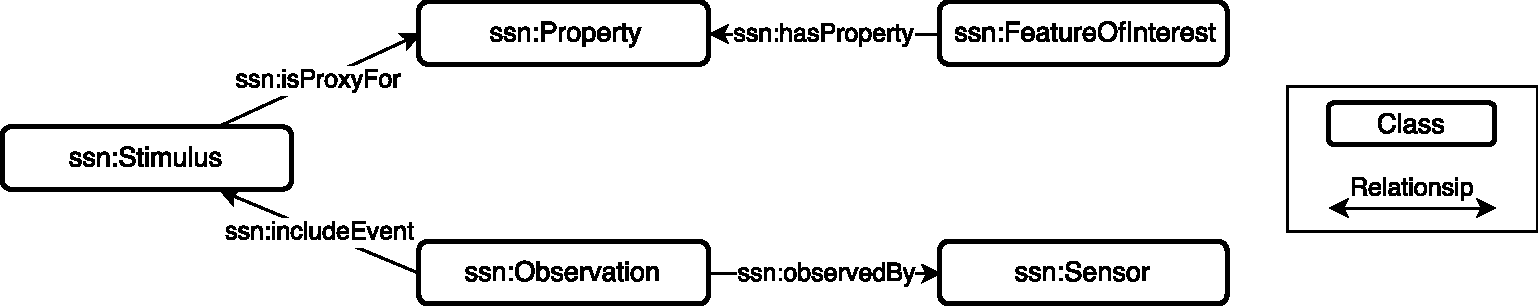
\includegraphics[width=1\textwidth]{ssn_ontology.pdf}
  \caption{Semantic Sensor Network (simplified) ontology}
  \label{fig:ssn_ontology}
\end{figure}

\subsubsection{Extending SSNO} \label{ssubsec:extended_ssno}
As far as it goes Brick and SSN are good ontologies for modeling a building and its sensor network, but in a Energy Management System (EMS) context, and for FDD applications in particular, it is essential to understand the cause-effect relationships in the building. In order to to that, IBM Research extended the SSNO through the introduction of additional classes and references as in \autoref{fig:extended_ssno}. phy:PhysicalProcess represents laws of physics through a simplified model. Different subclasses of physical processes are derived from LTI system processes and will be described in . % TODO later chapter
phy:FeatureLink tells which kind of relationship exist between two ssn:FeatureOfInterest, such a link could be a wall between two rooms or a window between a room and the outside. phy:Cause and phy:Effect are subclasses of ssn:Stimulus useful for differentiate whether said stimulus is a cause or an effect of a ssn:Observation. phy:Anomaly is a subclass of ssn:Observation, it describes out-of-range observations that need to be diagnosed, like a high temperature in a room. phy:ObservedCause is still a subclass of ssn:Observation; it is used for describing a measurment that can be a cause of an anomaly.

\begin{figure}
  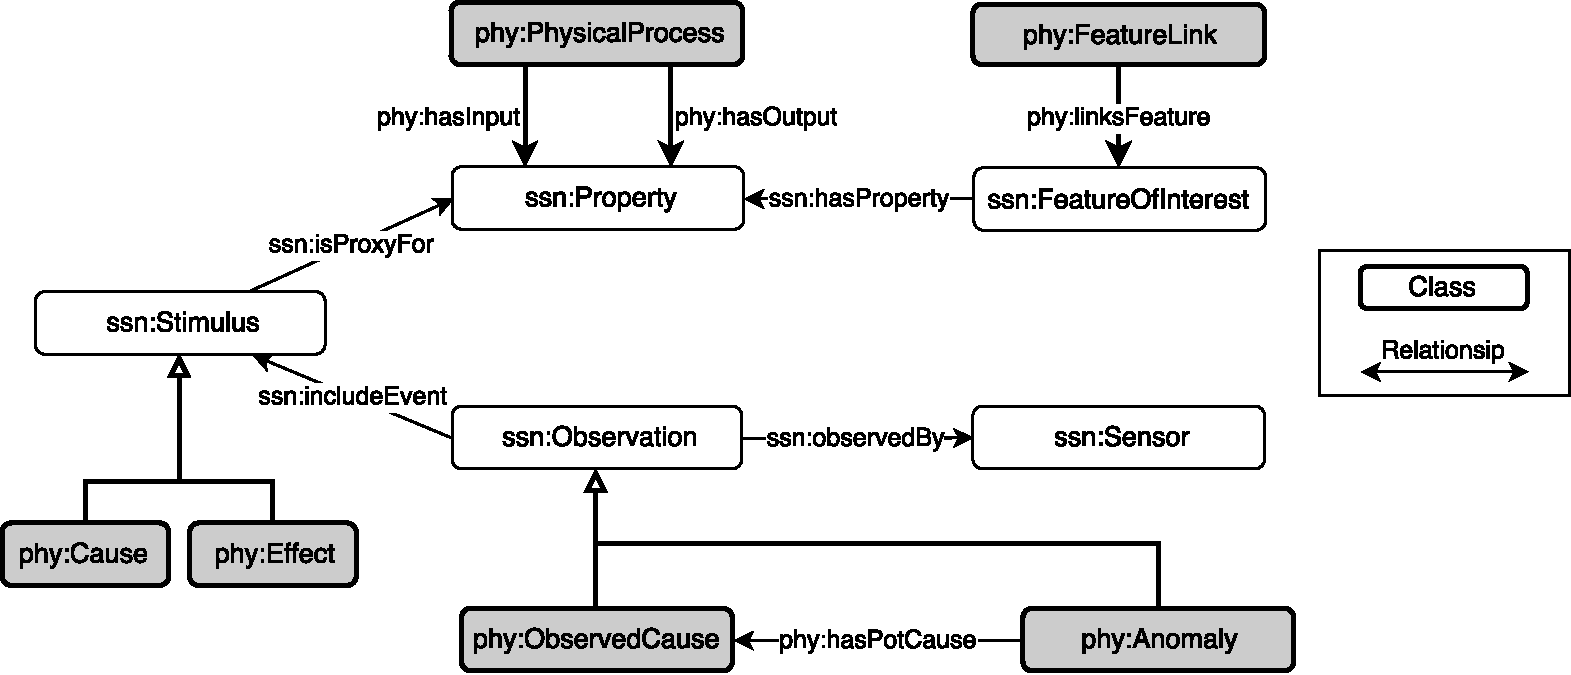
\includegraphics[width=1\textwidth]{extended_ssno.pdf}
  \caption{Extended SSN ontology. Extensions are highlighted with bold line and a light grey background.}
  \label{fig:extended_ssno}
\end{figure}
